\chapter{La biodiversité}\label{ch:g5:biodiversity}

Prends un mètre carré de prairie fleurie et mets-toi à compter~: une
douzaine de sortes de \omterm{def:g1:plants-around-us:plant}{plantes}, des scarabées et des punaises à n'en
plus finir, des araignées, des escargots, des vers en dessous et des
papillons au-dessus. Essaie maintenant le même mètre carré de cour
d'école bitumée. La différence entre ces deux comptes a un nom ---
la \omterm{def:g5:biodiversity:biodiversity}{biodiversité} --- et c'est devenu l'un des mots les plus importants
de la \omterm{def:g1:living-or-not:living}{biologie}.

\section{La diversité du vivant}

\begin{definition}[Espèce]\label{def:g5:biodiversity:species}
Une \emph{espèce}\index{espèce} est une sorte particulière d'\omterm{def:g1:living-or-not:living}{être
vivant}~: tous les individus bâtis sur le même modèle, et qui se
reproduisent entre eux. Le moineau domestique est une espèce~; la
pâquerette aussi, le renard roux, l'escargot des jardins. Les
classes de \cref{ch:g4:classifying-animals} sont des boîtes qui
contiennent de nombreuses espèces~: «~\omterm{prop:g3:sorting-living-things:groups}{mammifères}~» en abrite des
milliers.
\end{definition}

\begin{definition}[Biodiversité]\label{def:g5:biodiversity:biodiversity}
La \emph{biodiversité}\index{biodiversité} d'un lieu est la variété
de vie qu'il abrite --- avant tout, combien d'\emph{\omterm{def:g5:biodiversity:species}{espèces}}
différentes y vivent, et dans quel état chacune se porte. Une
prairie fleurie, riche en \omterm{def:g5:biodiversity:species}{espèces}, a une forte biodiversité~; une
cour bitumée, presque aucune.
\end{definition}

\begin{omfigure}
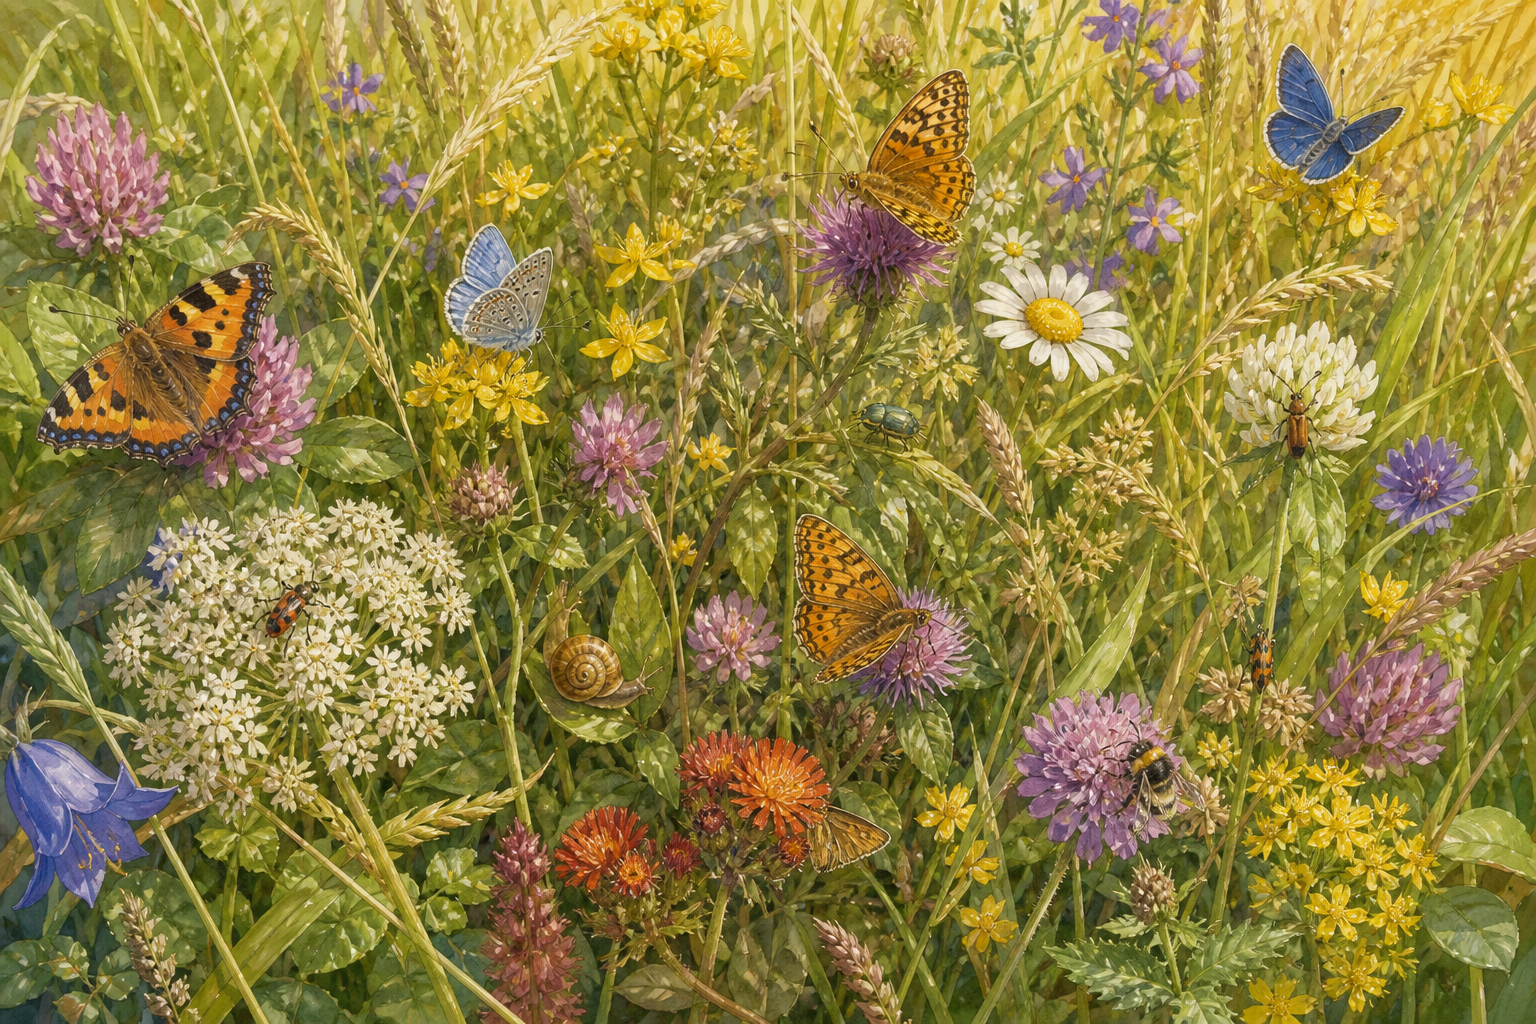
\includegraphics[width=0.62\linewidth]{images/book1/ai/g5-biodiversity-meadow.png}

{\small Un mètre carré de prairie, comptage en cours~: des herbes,
des \omterm{def:g3:flowers-fruits-seeds:parts}{fleurs}, des papillons, des scarabées, un escargot --- et le
comptage commence à peine.}
\end{omfigure}

\begin{example}[Compter la planète]\label{ex:g5:biodiversity:planet}
Les scientifiques ont nommé environ deux millions d'\omterm{def:g5:biodiversity:species}{espèces} jusqu'ici
--- et sont sûrs que ce n'est qu'une partie du total, car chaque
expédition sérieuse trouve de nouvelles \omterm{def:g5:biodiversity:species}{espèces}~: des scarabées
surtout (aucun groupe n'a plus d'\omterm{def:g5:biodiversity:species}{espèces} nommées), mais aussi des
\omterm{prop:g3:sorting-living-things:groups}{poissons}, des grenouilles, des \omterm{def:g1:plants-around-us:plant}{plantes}, et même parfois des
\omterm{prop:g3:sorting-living-things:groups}{mammifères}. Le nombre total d'\omterm{def:g5:biodiversity:species}{espèces} de la Terre reste inconnu ---
la plupart des estimations donnent des millions au-delà de ce qui
est nommé.
\end{example}

\begin{remark}[La diversité à toutes les échelles]\label{rem:g5:biodiversity:scales}
La \omterm{def:g5:biodiversity:biodiversity}{biodiversité} se montre à plusieurs échelles à la fois~: beaucoup
d'\omterm{def:g5:biodiversity:species}{espèces} dans un même milieu~; beaucoup de milieux différents \omterm{def:g3:bones-and-muscles:skeleton}{côte} à
\omterm{def:g3:bones-and-muscles:skeleton}{côte} (mare, haie, pré --- chacun avec ses \omterm{def:g5:biodiversity:species}{espèces}, comme le montrait
\cref{ex:g2:where-animals-live:four})~; et, à l'intérieur d'une même
\omterm{def:g5:biodiversity:species}{espèce}, pas deux individus tout à fait pareils --- pas deux escargots
des jardins ne portent exactement la même \omterm{def:g1:animals-around-us:covering}{coquille}. De la variété
dans de la variété dans de la variété.
\end{remark}

\section{Pourquoi la biodiversité compte}

\begin{proposition}[Le réseau a besoin de ses fils]\label{prop:g5:biodiversity:web}
Les \omterm{def:g5:biodiversity:species}{espèces} d'un milieu se nourrissent, s'abritent, se pollinisent et
se nettoient les unes les autres --- ce sont les fils d'un même
réseau (\cref{rem:g3:food-chains:web}). Un réseau riche, à
nombreux fils, encaisse un choc~: si une \omterm{def:g5:biodiversity:species}{espèce} proie vient à
manquer, ses chasseurs passent à d'autres. Un réseau pauvre se
déchire vite~: chaque \omterm{def:g5:biodiversity:species}{espèce} perdue laisse aux survivants moins de
solutions. La \omterm{def:g5:biodiversity:biodiversity}{biodiversité} est la solidité du réseau.
\end{proposition}
\admitted

\begin{example}[L'épreuve du verger]\label{ex:g5:biodiversity:orchard}
Un verger avec des haies, des bandes de \omterm{def:g3:flowers-fruits-seeds:parts}{fleurs} sauvages et de vieux
arbres héberge des dizaines d'\omterm{def:g5:biodiversity:species}{espèces} auxiliaires~: abeilles et
syrphes pollinisent les \omterm{def:g3:flowers-fruits-seeds:parts}{fleurs}
(\cref{rem:g3:flowers-fruits-seeds:bees}), coccinelles mangent les
pucerons, \omterm{prop:g3:sorting-living-things:groups}{oiseaux} patrouillent à la recherche des \omterm{ex:g2:animals-grow-up:butterfly}{chenilles}, vers
gardent le sol ouvert. Arrache les haies et fauche les \omterm{def:g3:flowers-fruits-seeds:parts}{fleurs}, et
les auxiliaires s'en vont --- l'arboriculteur doit alors faire seul
leur travail, un travail que le réseau faisait gratuitement.
\end{example}

\begin{example}[Les humains vivent du réseau]\label{ex:g5:biodiversity:people}
Tout ce que les humains mangent remonte à des \omterm{def:g5:biodiversity:species}{espèces} vivantes
(\cref{rem:g4:what-plants-need:everyone})~; la plupart de nos
médicaments ont d'abord été trouvés dans des \omterm{def:g1:plants-around-us:plant}{plantes}, des
moisissures et d'autres \omterm{def:g1:living-or-not:living}{êtres vivants}~; le coton, la laine, le bois
et le cuir sont des produits d'\omterm{def:g5:biodiversity:species}{espèces}. Les fils du réseau traversent
tout droit chaque cuisine, chaque pharmacie et chaque armoire.
\end{example}

\section{La biodiversité peut se perdre --- et se soutenir}

\begin{proposition}[Comment la diversité se perd]\label{prop:g5:biodiversity:loss}
Une \omterm{def:g5:biodiversity:species}{espèce} s'amenuise quand on lui retire ce dont elle dépend~:
\begin{itemize}
  \item son \emph{\omterm{def:g2:where-animals-live:habitat}{milieu de vie}} détruit --- la mare asséchée de
        \cref{prop:g2:where-animals-live:loss}, la haie arrachée,
        le pré bitumé~;
  \item son \omterm{def:g2:caring-for-nature:environment}{environnement} empoisonné --- déchets et produits
        chimiques (\cref{prop:g2:caring-for-nature:harm})~;
  \item trop de prélèvements --- surpêche, cueillette excessive,
        chasse excessive.
\end{itemize}
Une \omterm{def:g5:biodiversity:species}{espèce} entièrement disparue --- partout, pour toujours --- est
\emph{éteinte}\index{éteinte}. L'extinction n'est pas comme une
partie perdue~: il n'y a pas de manche suivante.
\end{proposition}
\admitted

\begin{method}[Soutenir la biodiversité, en commençant petit]\label{met:g5:biodiversity:help}
Les recettes de \cref{met:g2:caring-for-nature:rules} changent
d'échelle~:
\begin{enumerate}
  \item garde et \omterm{def:g1:plants-around-us:plant}{plante} de la variété --- une haie de cinq
        arbustes vaut mieux qu'une clôture, une bande fleurie
        mieux que du gravier nu~;
  \item laisse des coins sauvages~: bois mort, tas de \omterm{def:g1:plants-around-us:parts}{feuilles},
        herbe non tondue sont des milieux de vie
        (\cref{ex:g2:caring-for-nature:home})~;
  \item aide les auxiliaires~: nichoirs, abris à \omterm{prop:g3:sorting-living-things:groups}{insectes}, une
        mare même minuscule
        (\cref{ex:g2:where-animals-live:schoolpond})~;
  \item compte ce qui vit autour de toi, année après année ---
        ce qu'on compte, on le remarque, et ce qu'on remarque
        finit protégé.
\end{enumerate}
\end{method}

\begin{example}[Le retour des cigognes]\label{ex:g5:biodiversity:storks}
Là où des prairies humides ont été restaurées et des plateformes de
nid installées, les cigognes --- presque disparues de régions
entières --- sont revenues nicher, et avec elles les grenouilles,
les libellules et les \omterm{def:g3:flowers-fruits-seeds:parts}{fleurs} des prés. Les \omterm{def:g5:biodiversity:species}{espèces} reviennent quand
on renoue leurs fils~: la protection marche, et ses résultats
s'observent depuis la place du village.
\end{example}

\section{Exercices}

\begin{exercise}[$\star$]\label{exo:g5:biodiversity:1}
Qu'est-ce qu'une \omterm{def:g5:biodiversity:species}{espèce}~? Donne trois exemples tirés de ce chapitre.
\end{exercise}

\begin{exercise}[$\star$]\label{exo:g5:biodiversity:2}
Qu'est-ce que la \omterm{def:g5:biodiversity:biodiversity}{biodiversité}~? Compare la prairie et la cour
bitumée.
\end{exercise}

\begin{exercise}[$\star$]\label{exo:g5:biodiversity:3}
Combien d'\omterm{def:g5:biodiversity:species}{espèces} sont nommées à ce jour, à peu près~? Pourquoi le
vrai nombre est-il certainement plus grand~?
\end{exercise}

\begin{exercise}[$\star$]\label{exo:g5:biodiversity:4}
Nomme les trois échelles de diversité de
\cref{rem:g5:biodiversity:scales}, chacune avec son exemple.
\end{exercise}

\begin{exercise}[$\star$]\label{exo:g5:biodiversity:5}
Pourquoi un réseau riche en \omterm{def:g5:biodiversity:species}{espèces} survit-il mieux aux chocs qu'un
réseau pauvre~? Sers-toi de l'argument des chasseurs qui changent de
proie.
\end{exercise}

\begin{exercise}[$\star$]\label{exo:g5:biodiversity:6}
Énumère quatre \omterm{def:g5:biodiversity:species}{espèces} auxiliaires du verger et le travail gratuit
que fait chacune.
\end{exercise}

\begin{exercise}[$\star$]\label{exo:g5:biodiversity:7}
Donne les trois façons dont une \omterm{def:g5:biodiversity:species}{espèce} s'amenuise, avec un exemple
pour chacune. Que veut dire \emph{\omterm{prop:g5:biodiversity:loss}{éteinte}}~?
\end{exercise}

\begin{exercise}[$\star$]\label{exo:g5:biodiversity:8}
À toi d'essayer~: compte les \omterm{def:g5:biodiversity:species}{espèces} --- \omterm{def:g1:plants-around-us:plant}{plantes} et \omterm{def:g1:animals-around-us:animal}{animaux}, nommés
ou décrits --- dans un petit carré que tu choisis dehors. Compte
ensuite un carré bitumé pour comparer. Tes deux nombres sont une
mesure de \omterm{def:g5:biodiversity:biodiversity}{biodiversité}.
\end{exercise}

\begin{exercise}[$\star\star$]\label{exo:g5:biodiversity:9}
«~Perdre une espèce de scarabée sur des milliers ne peut pas
compter.~» Réponds avec \cref{prop:g5:biodiversity:web} --- et avec
le fait que personne ne connaît tous les fils que tient une \omterm{def:g5:biodiversity:species}{espèce}.
\end{exercise}

\begin{exercise}[$\star\star$]\label{exo:g5:biodiversity:10}
L'histoire des cigognes est présentée comme une réussite de la
protection des \emph{milieux} plutôt que de la protection des
cigognes une par une. Explique la différence, en utilisant
\cref{prop:g2:where-animals-live:loss} et ce qui est revenu en même
temps que les cigognes.
\end{exercise}

\begin{exercise}[$\star\star\star$]\label{exo:g5:biodiversity:11}
Un arboriculteur remplace haies et bandes fleuries par des clôtures
et du gravier, puis doit louer des ruches pour la pollinisation et
traiter contre les pucerons --- en dépensant de l'argent pour des
travaux autrefois gratuits. Sers-toi de
\cref{ex:g5:biodiversity:orchard} pour expliquer ce qui a vraiment
été retiré --- et pourquoi les comptes du travail gratuit de la
nature n'apparaissent d'ordinaire qu'une fois qu'il s'arrête.
\end{exercise}
